%%%%%%%%%%%%%%%%%%%%%%%%%%%%%%%%%%%%%%%%%
% Beamer Presentation
% LaTeX Template
% Version 1.0 (10/11/12)
%
% This template has been downloaded from:
% http://www.LaTeXTemplates.com
%
% License:
% CC BY-NC-SA 3.0 (http://creativecommons.org/licenses/by-nc-sa/3.0/)
%
%%%%%%%%%%%%%%%%%%%%%%%%%%%%%%%%%%%%%%%%%

%----------------------------------------------------------------------------------------
%	PACKAGES AND THEMES
%----------------------------------------------------------------------------------------

\documentclass{beamer}

\mode<presentation> {
\usetheme{Madrid}
}
\usepackage{adjustbox}
\usepackage{graphicx} % Allows including images
\usepackage{booktabs} % Allows the use of \toprule, \midrule and \bottomrule in tables

%----------------------------------------------------------------------------------------
%	TITLE PAGE
%----------------------------------------------------------------------------------------

\title[Comparison of classifiers]{A comparison Of classifiers for oil spill detection} % The short title appears at the bottom of every slide, the full title is only on the title page

\institute[TUDelft] % Your institution as it will appear on the bottom of every slide, may be shorthand to save space
{
Delft University of Technology \\ % Your institution for the title page
\medskip
%\textit{john@smith.com} % Your email address
}
\date{30$^{th}$ October 2014} 
\author{Andy\\ Thomas\\ Soheil} % Your name

\begin{document}

\begin{frame}
\titlepage % Print the title page as the first slide
\end{frame}

\begin{frame}
\frametitle{Overview} % Table of contents slide, comment this block out to remove it
\begin{enumerate}
	\item Introduction
	\item Oil Spill Detection
	\item SAR Images	
	\item Typical Problems
	\item SAR Preprocessing
	\item Features \& Selection
	\item Summary of Classifiers 
	\item Our Research
	\item Recommendations \& Conclusion
\end{enumerate}

%\tableofcontents % Throughout your presentation, if you choose to use \section{} and \subsection{} commands, these will automatically be printed on this slide as an overview of your presentation
\end{frame}

%----------------------------------------------------------------------------------------
%	PRESENTATION SLIDES
%----------------------------------------------------------------------------------------

%------------------------------------------------
%\section{First Section} % Sections can be created in order to organize your presentation into discrete blocks, all sections and subsections are automatically printed in the table of contents as an overview of the talk
%------------------------------------------------

%\subsection{Subsection Example} % A subsection can be created just before a set of slides with a common theme to further break down your presentation into chunks

\begin{frame}
\frametitle{Introduction}
\begin{columns}[T]
    \begin{column}{.5\textwidth}
     
		\begin{itemize}
			\item What is an oil spill?
			\item Why is of importance to detect oil spill? %enviornmental pollution,BP pais 27 bilion for cleanup in gulf of mexico
			\item How to detect oil spills? %SAR image, difference of Oil spill & lookalike
			
			
		\end{itemize}
   
    \end{column}
    \begin{column}{.5\textwidth}
    
% Your image included here
	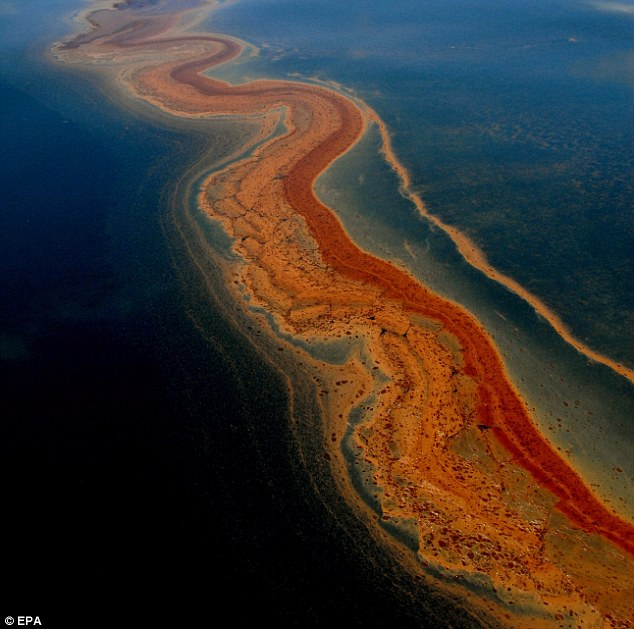
\includegraphics[width=60mm,scale=1]{./img/mex.jpg}	    
	
    \end{column}
  \end{columns}
\end{frame}

\begin{frame}
\frametitle{General oil spill detection approach}
\begin{figure}
	\centering
    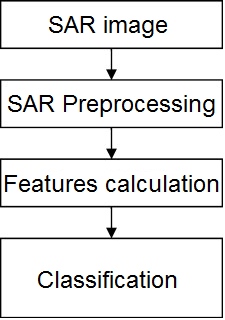
\includegraphics[width=40mm,scale=1]{./img/basicsteps.png}
\end{figure}



\end{frame}
%------------------------------------------------
\begin{frame}
\frametitle{SAR image}
\begin{itemize}
	\item Has high resolution
	\item Can monitor ocean 24 hours a day
	\item Covers large area 

\end{itemize}
\end{frame}

%------------------------------------------------

\begin{frame}
\frametitle{Typical problems}
\begin{itemize}
	\item Lookalikes
	\item Imbalanced dataset
	\item Data is scarce
	\item Noise
	\item Gathering contextual features
	
\end{itemize}
\end{frame}


%------------------------------------------------

\begin{frame}
\frametitle{SAR preprocessing}
\begin{figure}
	\centering
    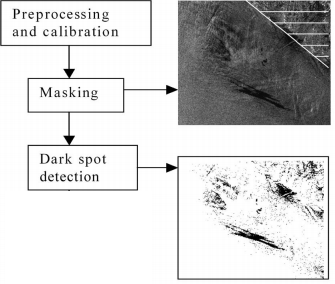
\includegraphics[width=60mm,scale=1]{./img/preprocessing_diagram.png}
\end{figure}
\end{frame}

%------------------------------------------------

\begin{frame}
\frametitle{Features}
\begin{itemize}
	\item What are features?
	\item Types of features \begin{itemize}
					\item Geometrical %area,perimeter, complexity
					\item Physical %mean, max backscatter value
					\item Texture %mean,contrast
					\item Contextual  %distance between dark spots
					\end{itemize}
				
\end{itemize}

\end{frame}

%------------------------------------------------

\begin{frame}
\frametitle{Feature Selection}
\begin{itemize}
	\item Choosing features
	\item Over fitting 
	\item Curse of dimensionality
\end{itemize}
\begin{figure}
	\centering
    \includegraphics[width=60mm,scale=1.5]{./img/overfit.png}
\end{figure}
\end{frame}
%-----------------------------------------

\begin{frame}
\frametitle{Supervised learning}

\begin{figure}
	\centering
    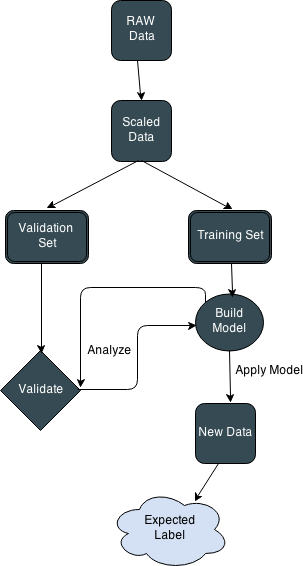
\includegraphics[width=40mm,scale=1]{./img/SL.png}
\end{figure}

\end{frame}

%------------------------------------------------

\begin{frame}
\frametitle{Support vector machines}
\begin{figure}
	\centering
    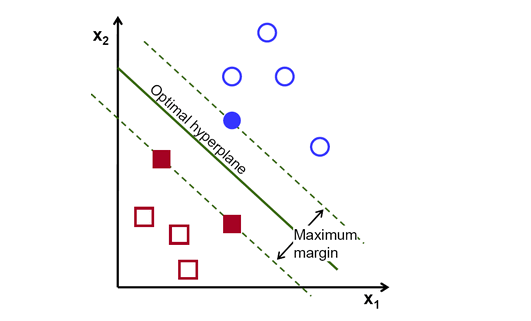
\includegraphics[width=90mm,scale=1]{./img/SVM.png}
\end{figure}

\end{frame}

%------------------------------------------------

\begin{frame} % Need to use the fragile option when verbatim is used in the slide
\frametitle{Decision Tree}
\begin{figure}
	\centering
    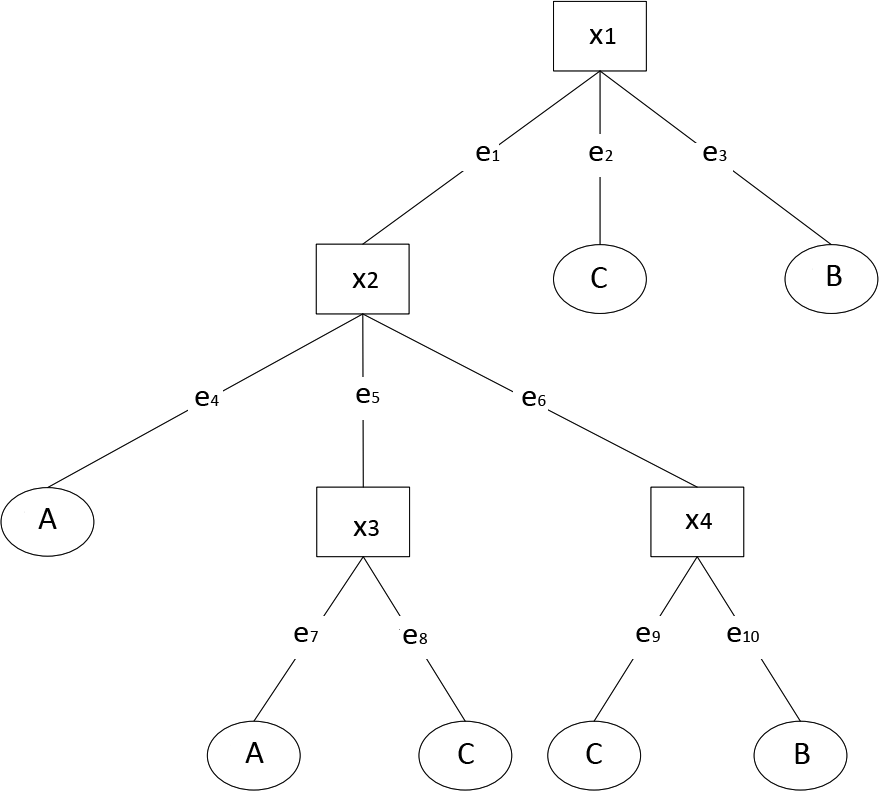
\includegraphics[width=70mm,scale=1]{./img/decisiontree.png}
\end{figure}

\end{frame}

%------------------------------------------------
\begin{frame} % Need to use the fragile option when verbatim is used in the slide
\frametitle{Perceptron}
\begin{figure}
	\centering
    
\includegraphics[width=\textwidth]{./img/perceptron.png}
\end{figure}

\end{frame}
\begin{frame}
\frametitle{Multi layer perceptrons}
\begin{figure}
	\centering
    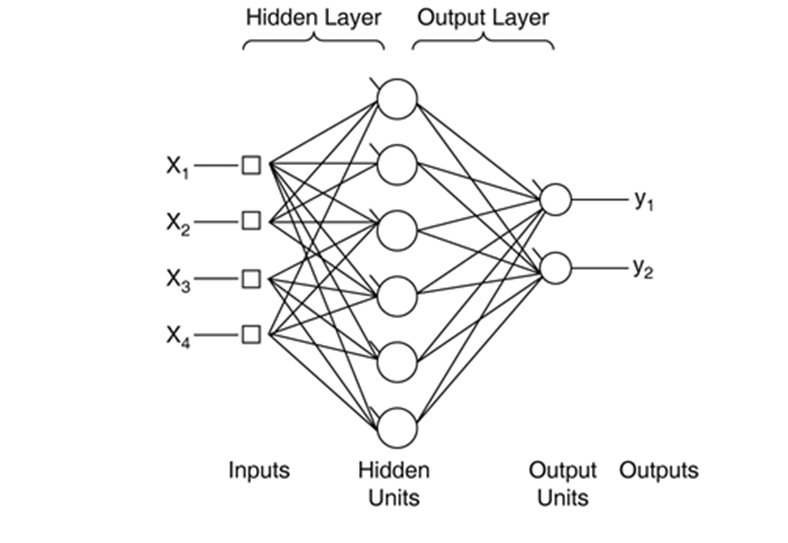
\includegraphics[width=90mm,scale=1]{./img/MLP.jpg}
\end{figure}
\end{frame}


%------------------------------------------------

\begin{frame}
\frametitle{Research goals}
\begin{itemize}
	\item Accuracy comparison
	\item Classifier characteristics vs field specific problems
	 
\end{itemize}
\end{frame}

%------------------------------------------------

\begin{frame}
\frametitle{Difficulties researching}
\begin{itemize}
	\item SVM was hardly used
	\item Not all details were specified
	\item Use of different datasets (unverified samples)
	\item Use of different features
	\item Free lunch theorem	 

\end{itemize}
\end{frame}

%------------------------------------------------

\begin{frame}
\frametitle{Fail}

\centerline{We did not manage to compare our three classifiers}

\end{frame}

%------------------------------------------------

\begin{frame}
\frametitle{The best classifier?}
\begin{itemize}
	\item Different accuracy in different situations
	\item SVM and MLP for large datasets
	\item SVM and MLP for non-linear cases
	\item DT for small datasets
	\item DT easiest to interpret
	
\end{itemize}
\end{frame}

%------------------------------------------------
\begin{frame}
\frametitle{Recommendations}
\begin{itemize}
	\item More research on SVM
	\item More research on Random Forest
	\item Shared database
	\item Bagging
	\item Image fusion

\end{itemize}
\end{frame}

%------------------------------------------------

\begin{frame}
\frametitle{Summary}
\begin{itemize}
	\item Oil spill detection
	\item Classifiers
	\item Research
	\item Difficulties
	\item Recommendations

\end{itemize}
\end{frame}

%------------------------------------------------

\begin{frame}

\end{frame}

%----------------------------------------------------------------------------------------
\begin{frame}

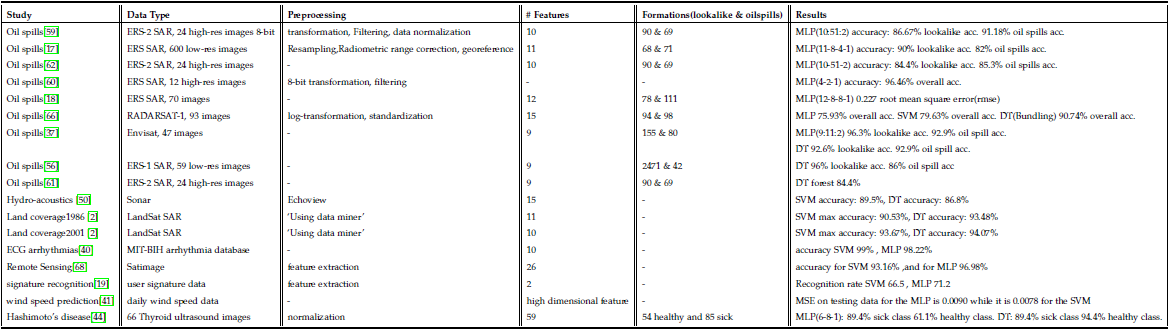
\includegraphics[width=\textwidth]{./img/table.png}

\end{frame}

%----------------------------------------------------------------------------------------
\begin{frame}
In case you need our credentials

A.S.Y.Chiu 1519360\\ T.P.van Helden 4106725\\ S.S.Jahanshahi 4127617


\end{frame}
%------------------------------------------------

\end{document} 